\documentclass{article}

\usepackage{amsmath}
\usepackage{minted}
\usepackage{graphicx}

\author{Austin Minor}
\title{Simulation Results of Channel Capacity using Parity Bits for Error Correction}
\date{\today}

\begin{document}
   \maketitle

   \section{Introduction}
      Claude Shannon was a major figure in creating the
      mathematical discipline of information theory. This
      paper analyzes how empirical results line up with
      the statements made by this mathematical model of
      information. More formally, we will be analyzing
      the effect of using parity bits for error correction
      and how well they are at approaching the formal limit
      on the conveyance of data.

      We will start with a mathematical description of the
      concepts related to the problem. From there, we will
      give the problem statement. After running the test,
      we will analyze the results and give our conclusion.
   \section{Mathematical Description}
      The official description of conveyable information
      is the mutual information between to system of events.
      Let $A$ be the source alphabet. Let $B$ be the reception
      alphabet. Let $Q$ be the transmission matrix (IE the
      probability of receiving $b_j \in B$ given a transmission
      of $a_i \in A$. Let these entries be represented as $q_{i,j}$
      respectively. For our example we will only consider the
      simpler channel known as the binary symmetric channel.
      Thus \[ Q =
      \begin{pmatrix}
         q_{0,0} & q_{0,1} \\
         q_{0,1} & q_{1,1}
      \end{pmatrix}
      =
      \begin{pmatrix}
         p & 1-p \\
         1-p & p
      \end{pmatrix}
      \]
      Given such a channel, the probability of bit errors
      can be represented by a Bernoulli Trial.

      The mutual information between two system of events (definition
      given elsewhere) is defined as following:
      \[
         I(A,B) =
         \sum_{i=1}^{m}
         \sum_{j=1}^{n}
         Pr(A_i \cup B_j)
         \log \left(\frac{Pr(A_i \cup B_j)}{Pr(A_i)Pr(B_j)}\right)
      \]
      \[
         ... =
         \sum_{i=1}^{m}
         Pr(A_i)
         \sum_{j=1}^{n}
         q_{i,j}
         \log \left(\frac{q_{i,j}}{\sum_{t=1}^{m} Pr(A_t) q_{t,j}}\right)
      \]
      It has been proved elsewhere that the maximal channel capacity
      (maximum I(A,B) based on $Pr(A_i)$ -- probability that a source letter
      is transmitted) for a BSC is when $Pr(A_1=0)=Pr(A_2=1)=\frac{1}{2}$.
      Furthermore for these values, 
      \[
      I(A,B) = p*log(2*p) + (1-p)*log(2*(1-p))
      \]
      For example, if $p = .99$ then $I(A,B) = .919$.
   \section{Problem Statement}
      To test this model of channel capacity and mutual information,
      a Matlab program was written that would satisfy the important
      requirements listed above ($Pr(A_i) = \frac{1}{2}$, Q as described above).

      The necessary error correction was implemented using parity bits.
      We implemented these using a message-packet model. Each message was
      composed of equal sized packets of information. Thus to each packet,
      we add a parity bit. From there the message is transmitted packet by
      packet until either an fixable error occurs, an unfixable error occurs,
      or the message is transmitted completely. In the first case, the packet
      is transmitted until it is received correctly or until a certain retry
      count (for us 20) is reached at which point the message is failed as
      in case two. In case two, negative one is returned to indicate a failure
      of transmission. To test the correctness
      of using parity bits, we included a counter
      to count the number of these errors incurred when transmitting.
      Furthermore, unfixable errors occur when the parity bit scheme
      fails to detect an error resulting in a flawed transmission. This
      can occur when more than one bit of a packet is errant.
      In the third case, the number of bits needed to transmit the message
      is recorded. After receiving this information, the number of bits
      needed to transmit the message is averaged over the number of successful
      transmissions unless this number is zero. For the case that it is zero,
      the number of bits remains zero. Next the channel capacity is computed
      by dividing the minimum bits needed from transmission by the actual
      number of bits used for transmission. This can be proved to give the
      channel capacity which we will not do. The Matlab code is below.

      \begin{listing}[H]
         \inputminted[linenos]{matlab}{../main.m}
         \caption{Main Simulator}
      \end{listing}
      
      \begin{listing}[H]
         \inputminted[linenos]{matlab}{../transmit.m}
         \caption{Transmission Simulator}
      \end{listing}

      \begin{listing}[H]
         \inputminted[linenos]{matlab}{../transmit_msg.m}
         \caption{Per-packet Transmission Simulator}
      \end{listing}

      \begin{listing}[H]
         \inputminted[linenos]{matlab}{../insert_parity_bit.m}
         \caption{Per-packet Parity Bit Inserter}
      \end{listing}

      \begin{listing}[H]
         \inputminted[linenos]{matlab}{../parity.m}
         \caption{Parity Bit Message Inserter}
      \end{listing}

      \begin{listing}[H]
         \inputminted[linenos]{matlab}{../generate_random_msg.m}
         \caption{Generator of Random Messages with Packets}
      \end{listing}
   \section{Analysis}
      \begin{figure}[H]
         \includegraphics[width=\textwidth]{images/polyline288.png}
         \caption{Results}
      \end{figure}
      \begin{figure}[H]
         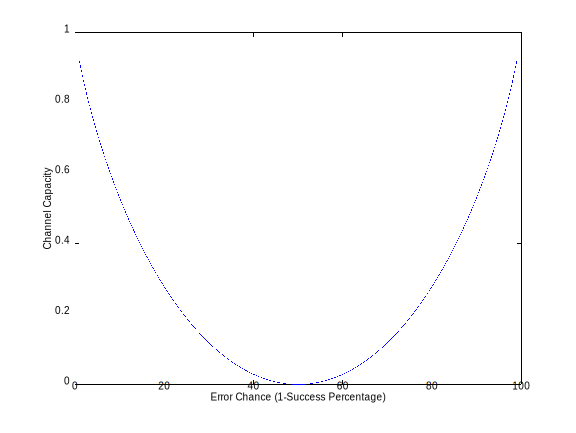
\includegraphics[width=\textwidth]{images/log.png}
         \caption{Theoretical Channel Capacity}
      \end{figure}
      Because the error correction was implemented using parity bits,
      the maximum channel capacity possible is $\frac{4}{5}$. This is since
      one new bit is added to each four bit transmission package thus lengthening
      the transmitted message at a $\frac{4}{5}$ rate.

      The average number of of bits needed follows a roughly linear pattern. This
      is of course till around 30 when the number of errors invalidates the
      scheme. It is of notice that around 25 the number of bits needed goes to
      0. From analysing the second graph on number of errant messages, we
      theorize that this tail end is due to the few times that message transmits
      successfully. Since this rarely happens after 20 according to the second
      graph, the tail end of the graph is less smooth and sporadic as the
      random events are smoothed over less and less successful transmissions.

      Since the goal of an error correction scheme is to reduce the number of
      errors to essentially zero, the second graph reveals that after 1\% error
      rate the number of errors is countable and is thus too much. Before 1\%
      the number of errors are not countable and the message is transmitted
      successfully. Further study of this can be done by modifying the Matlab
      code to print the actual vector of number of errors.

      Analyzing the first and third graph, shows the channel is relatively
      inefficient. Since the parity bit adds 1 bit of information for every 4 bits
      in our case, the channel capacity is low because we do not need this much
      information to detect and find errors. I.E. the max information at perfect
      transmission is $frac{4}{5}=80\%$.
      Furthermore, the channel capacity after 16 is less than 50\%.
      However, as mentioned in the second graph, the encoding
      schemes fails before the 16\% mark. The blips in the third graph,
      are theorized to arise from the same phenomenon explained earlier in
      relation to the sporadic tail of the number of bits needed for transmission.
      Also of note is the shape of the third graph. It seems to form either an
      inverse logarithmic shape or a hyperbolic shape. Thus given the definition
      of channel capacity above, the parity bit model does seem to follow
      similarly to the definition when compared to a plot of the optimal
      channel capacity function (excluding results after 50 which is due to
      a quality of the theoretical channel).
   \section{Conclusion}
      Parity bits are an easy to implement and fast method for detecting bits
      in a byte packet. They are fast in that the hardware can
      be implemented to do this kind of error checking because of its low
      computational complexity.
      However, they are not very efficient as noted. Not only
      that, they are not applicable in high noise environments since outside of
      1\% errors the parity scheme starts to fail to transmit properly in
      out example. However
      in low noise environments such as CPU to RAM, parity bits are a good scheme
      for quick, easily to implement error correction.
      
      Thanks goes to Pete Johnson, my teacher for Information Theory. Also
      to https://en.wikipedia.org/wiki/Parity\_bit for a description of parity
      bits and how they are calculated.
\end{document}
